\subsection{04 января. Старт, в. Перья}
\textit{Метеоусловия: днем температура $-8^{\circ}$, облачно}

\begin{figure}[h!]
	\centering
	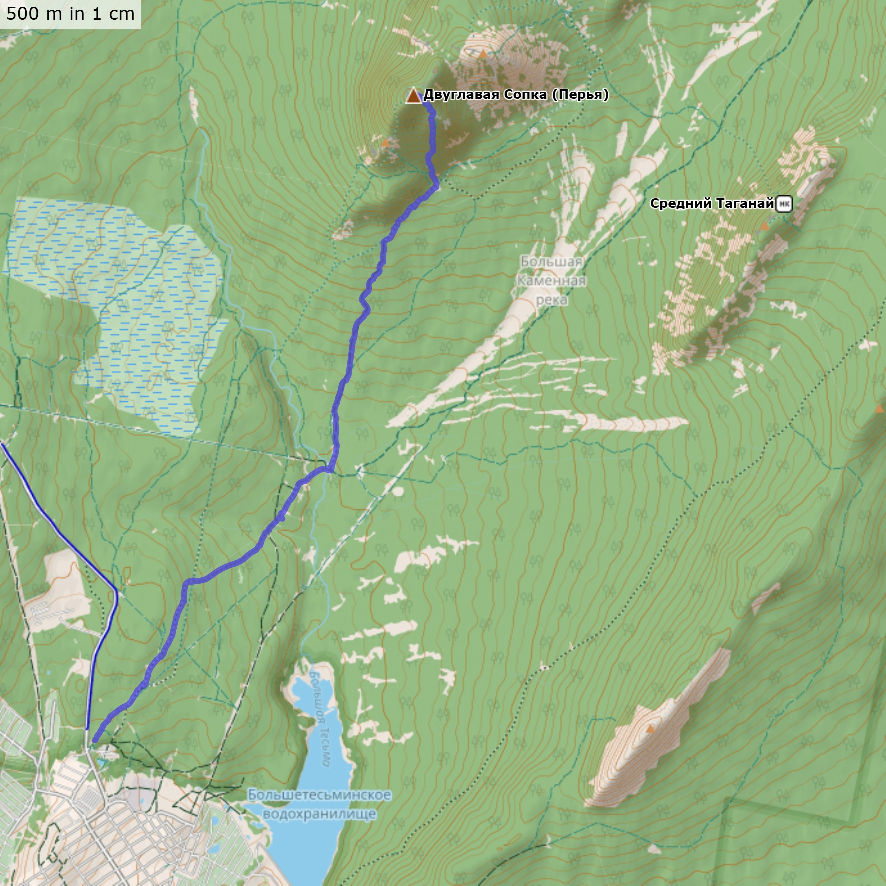
\includegraphics[angle=0, width=0.45\linewidth]{pics/maps/04}
	\label{fig:04}
\end{figure}

Прибыли на поезде в Златоуст в 4:12 впятером с большей частью снаряжения и еды. Пока ждали машину, распределили вещи по рюкзакам и успели покемарить.
К 8:50 приехал один из участников с родителями и в 2 плотных захода перевезли нас и всю кучу вещей.
Дождались в тепле оставшуюся часть группы, которая добиралась из Челябинска. Уже почти можно выдвигаться.

За полчаса распределили по весу снаряжение, коего оказалось больше, чем того бы хотелось. За это время руководитель заплатил за вход в нац. парк и зарегистрировал группу.

В последний раз поели домашней еды и в 10:42, наконец, вышли на маршрут. Дорога стартует прямо от усадьбы и отлично протоптана. По пути то и дело встречаются туристы и стоит много указателей, поэтому скучать не приходится.

\begin{figure}[h]
	\begin{minipage}[t]{0.49\linewidth}
		\centering
		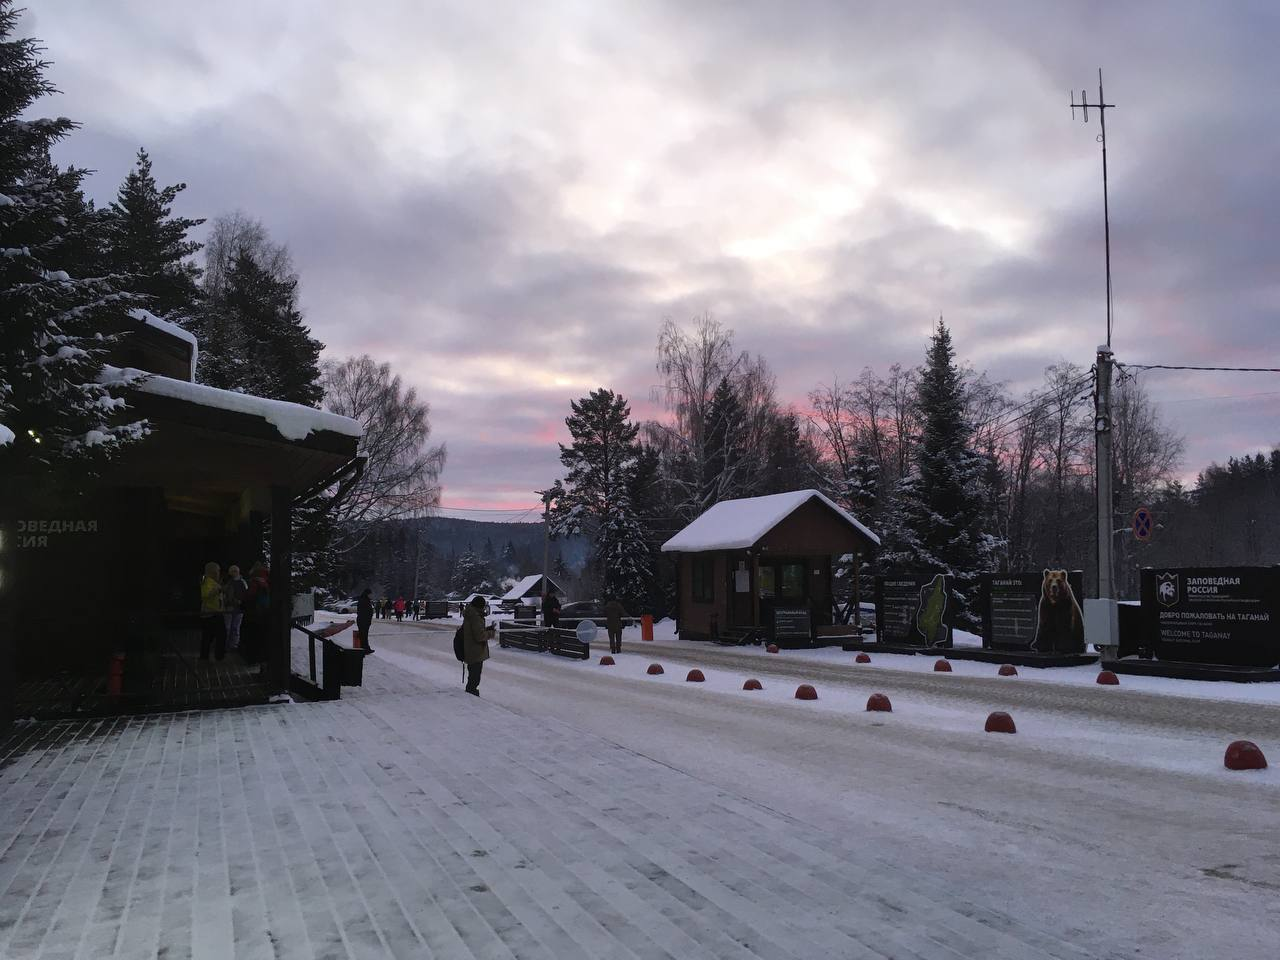
\includegraphics[width=\linewidth, height=5cm, keepaspectratio]{pics/04/central_estate.jpeg}
		\caption{Центральная усадьба. Вход в нац. парк Таганай}
		% \label{fig:central_estate.jpeg}
	\end{minipage}
	\hfill
	\begin{minipage}[t]{0.49\linewidth}
		\centering
		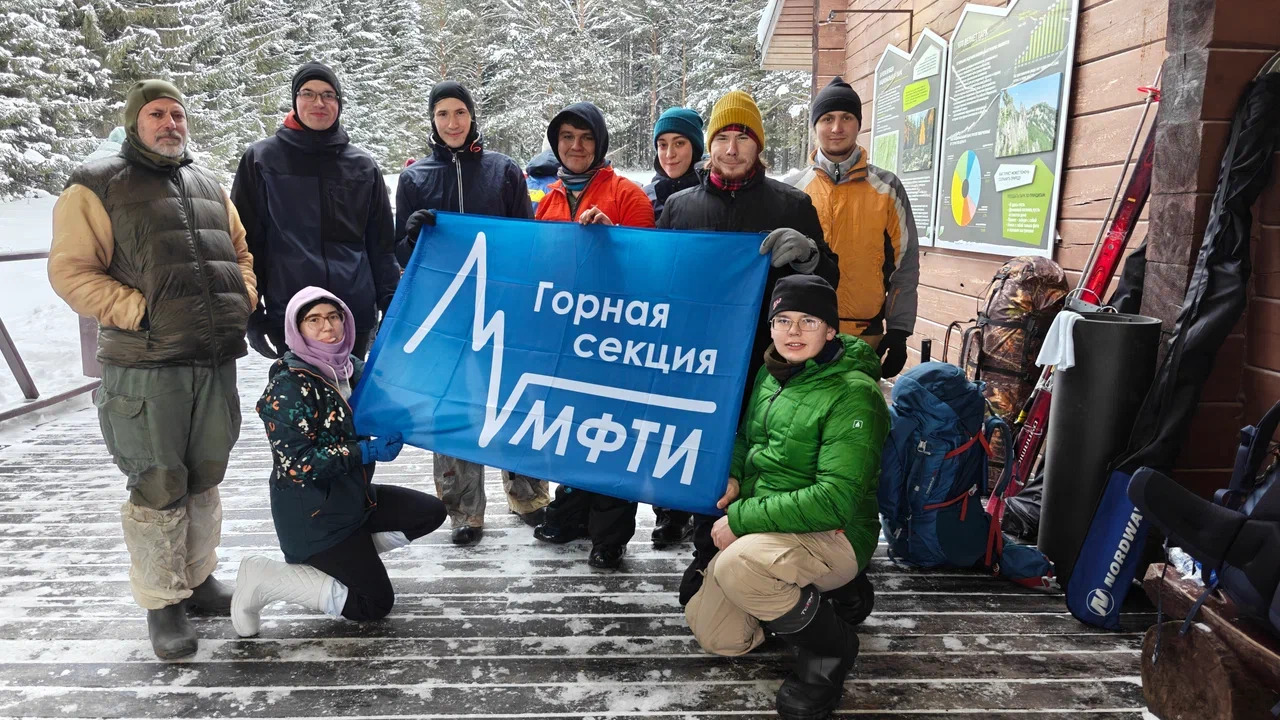
\includegraphics[width=\linewidth, height=5cm, keepaspectratio]{pics/04/start_04}
		\caption{Группа выходит. Лица светятся ярче}
		% \label{fig:start_04.jpg}
	\end{minipage}
	\label{fig:start}
\end{figure}

Скучать, собственно, никто не собирался, и уже в 11:15 у одного из участников отклеился камус на носке лыжи. Пока заклеили скотчем. Кто бы знал, что это только начало эпопеи.

В 11:40 на развилке Нижней и Верхней Таганайских троп встречные туристы сказали, что запланированный маршрут через Верхнюю тропу труднопроходим (особенно с лыжами) из-за того, что курумник там почти не закрыт снегом. Посовещались и решили идти сразу к приюту Белый ключ, а Перья взять радиально.

\begin{figure}[h!]
	\centering
	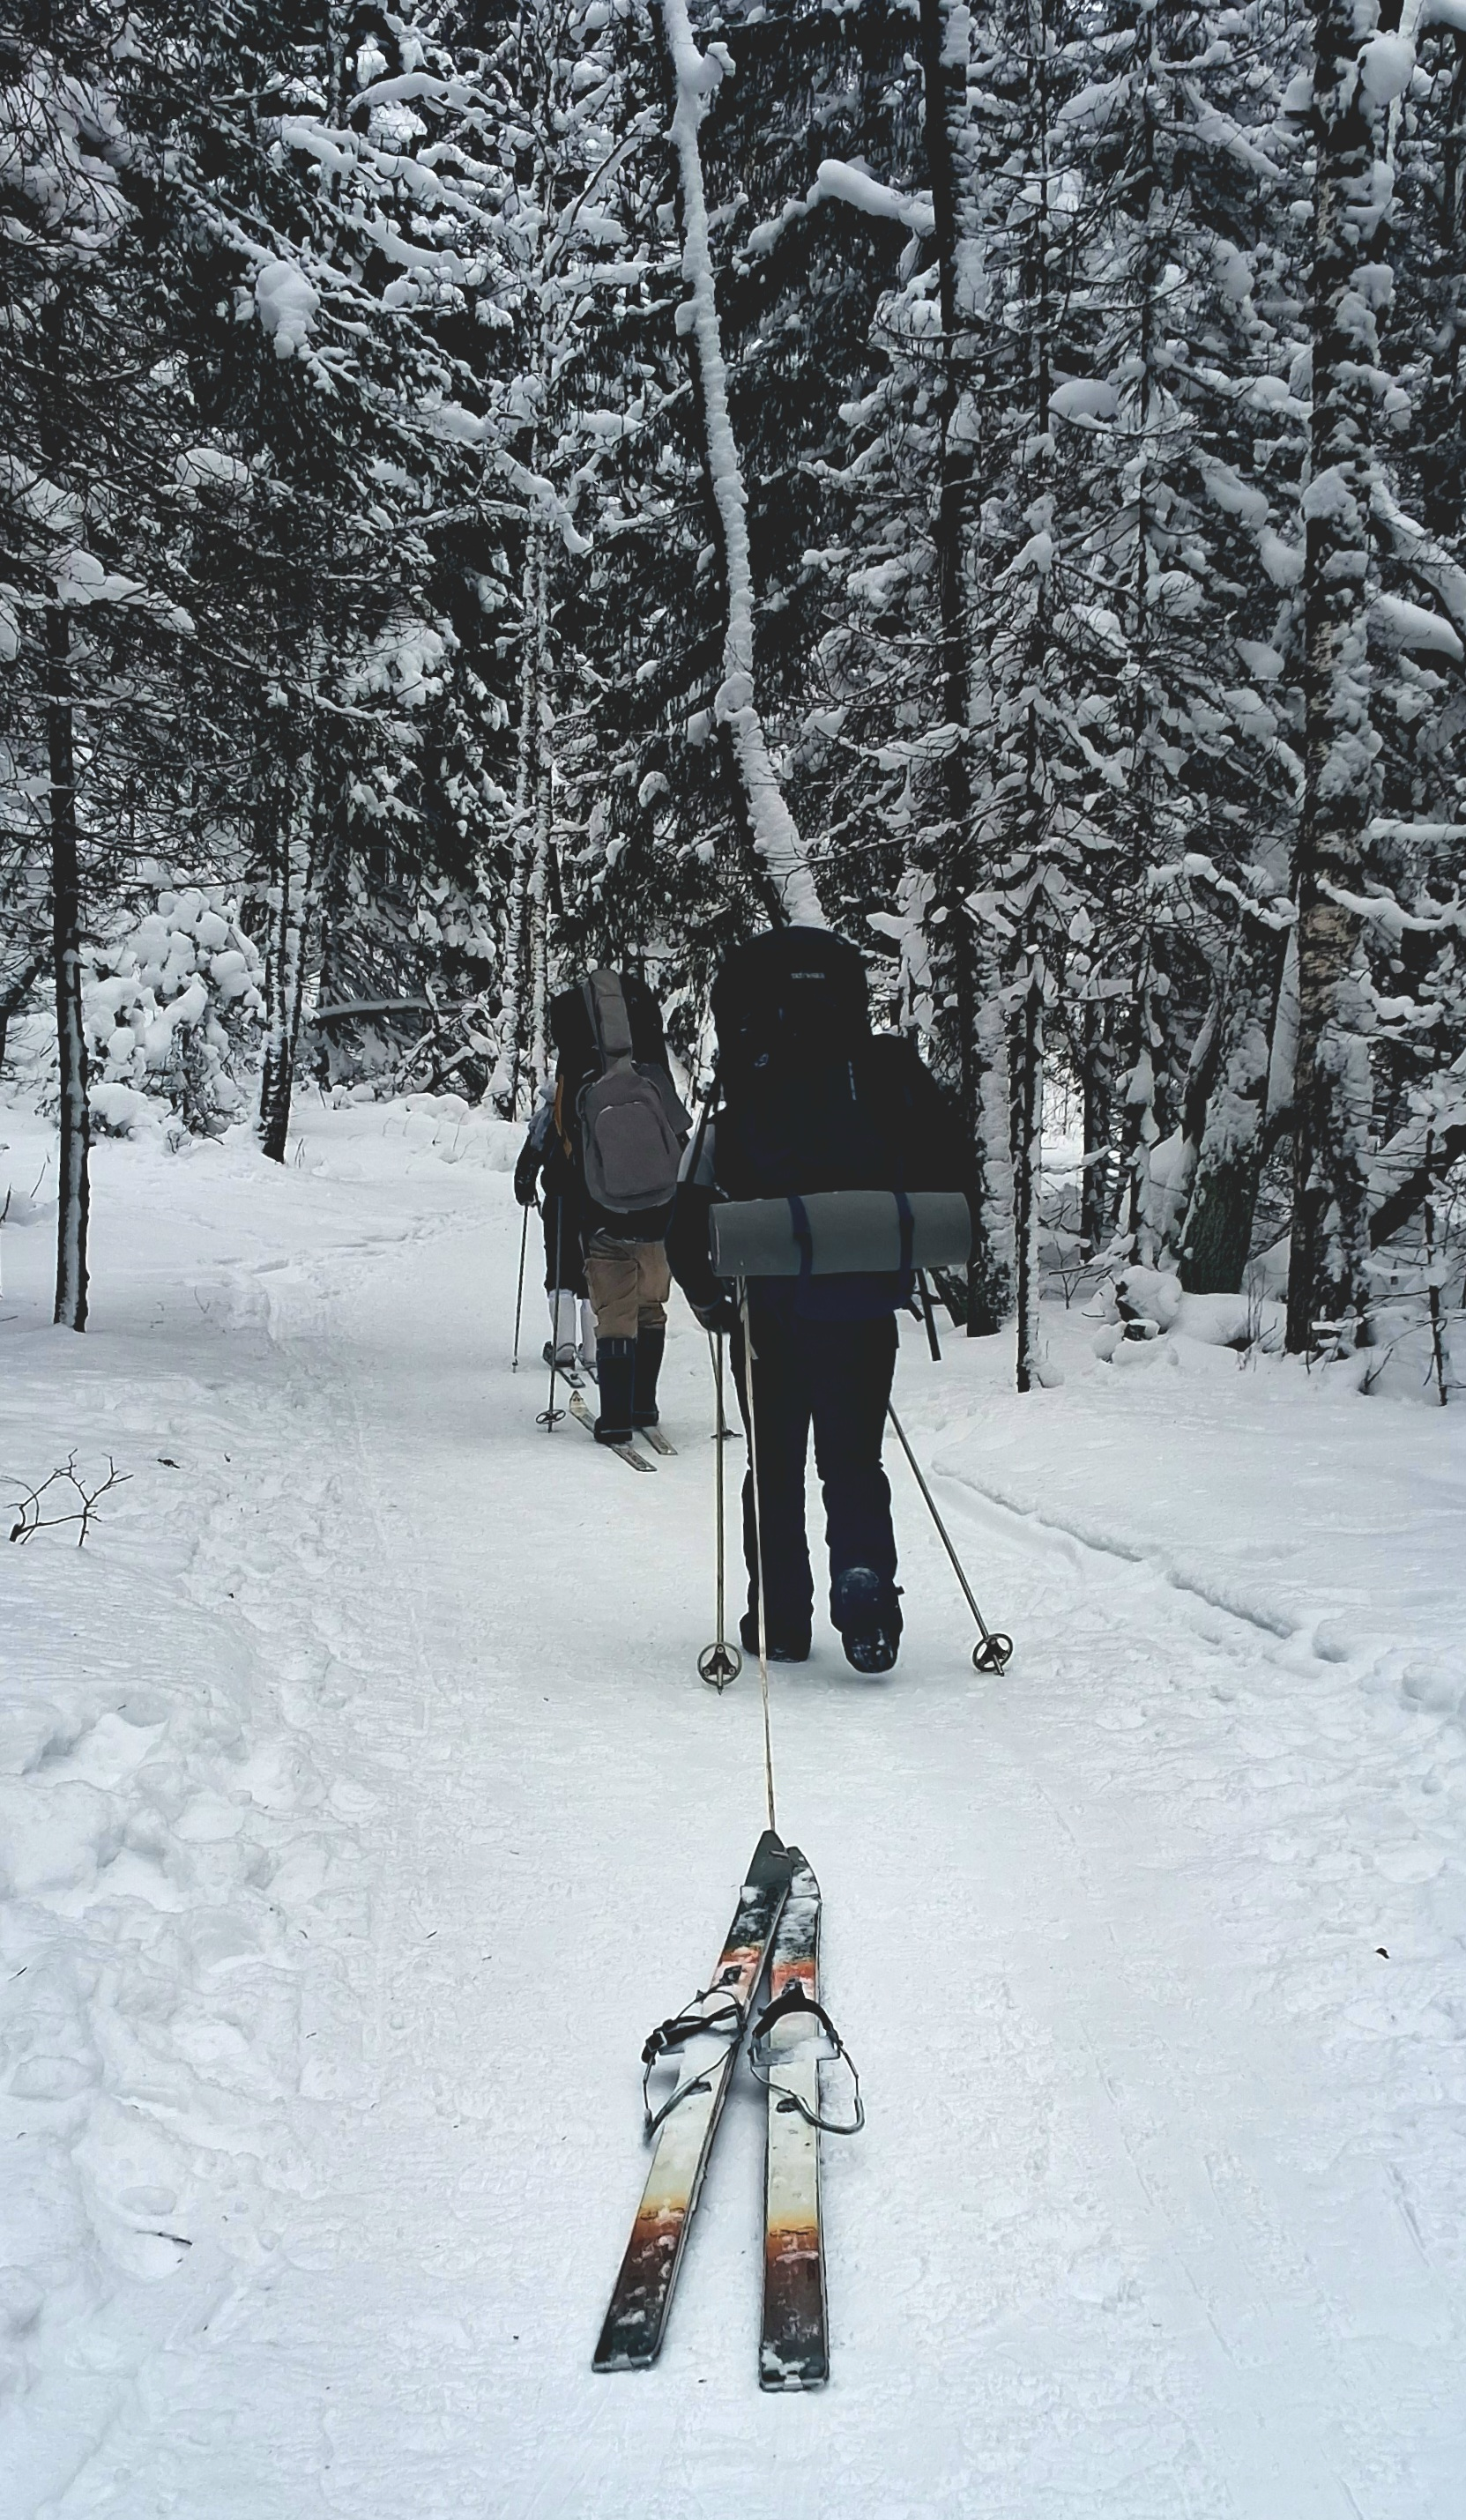
\includegraphics[angle=0, width=0.45\linewidth]{pics/04/near_Belyi_kliuch}
	\caption{На подступах к Белому ключу}
	\label{fig:near_Belyi_kliuch.jpg}
\end{figure}

Следующие 1.5 км до Железного моста спускались по приятному для катания на лыжах склону. Не всем, однако, спуск дался легко: ребята пока только привыкают к лыжам. Сделали небольшой привал и в 14:10 уже были на Белом ключе.
В приюте есть место под палатку чуть вдалеке от домиков, но мы решили ночевать в местной теплой палатке с печкой. Заплатили за стоянку 200 руб/чел, оставили вещи, и в 14:30 вышли на Перья. С собой взяли общую аптечку, флаг и шоколадку.

На первой части пути установлены лестницы, поэтому поднимались бодро (за 8 минут набрали 100 м!). Потом лестницы закончилась и темп сильно упал. Подниматься приходилось по уклону в $20^{\circ}$. Учились бить ступени ботинками в бахилах, а жизнь  осложнялась тем, что склон был раскатан несознательными гражданами.

\begin{figure}[h!]
	\centering
	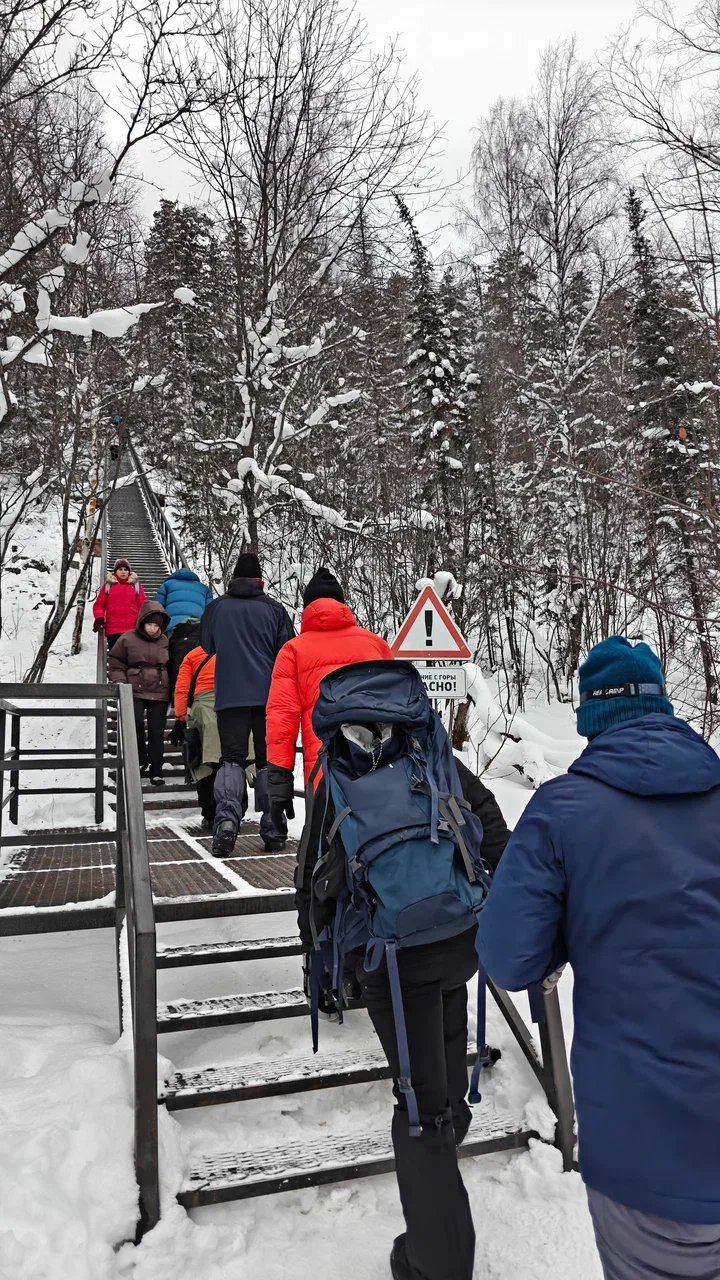
\includegraphics[angle=0, width=0.45\linewidth]{pics/04/perya_start}
	\caption{Бодро шагаем к Перьям}
	\label{fig:perya_start.jpg}
\end{figure}

В 15:20 группа выходит на выполаживание. Уже здесь появилась мобильная связь. Дальше склон чуть более пологий и в 15:42 мы на вершине.
С погодой нам не повезло: видимость оказалась низкая. Сами <<перья>>, однако, в тумане выглядят еще внушительнее. Налюбоваться успели, хотя на вершине нас и задул ветер. Спрятались от него за камнями. Теперь надо спускаться.

\begin{figure}[h!]
	\centering
	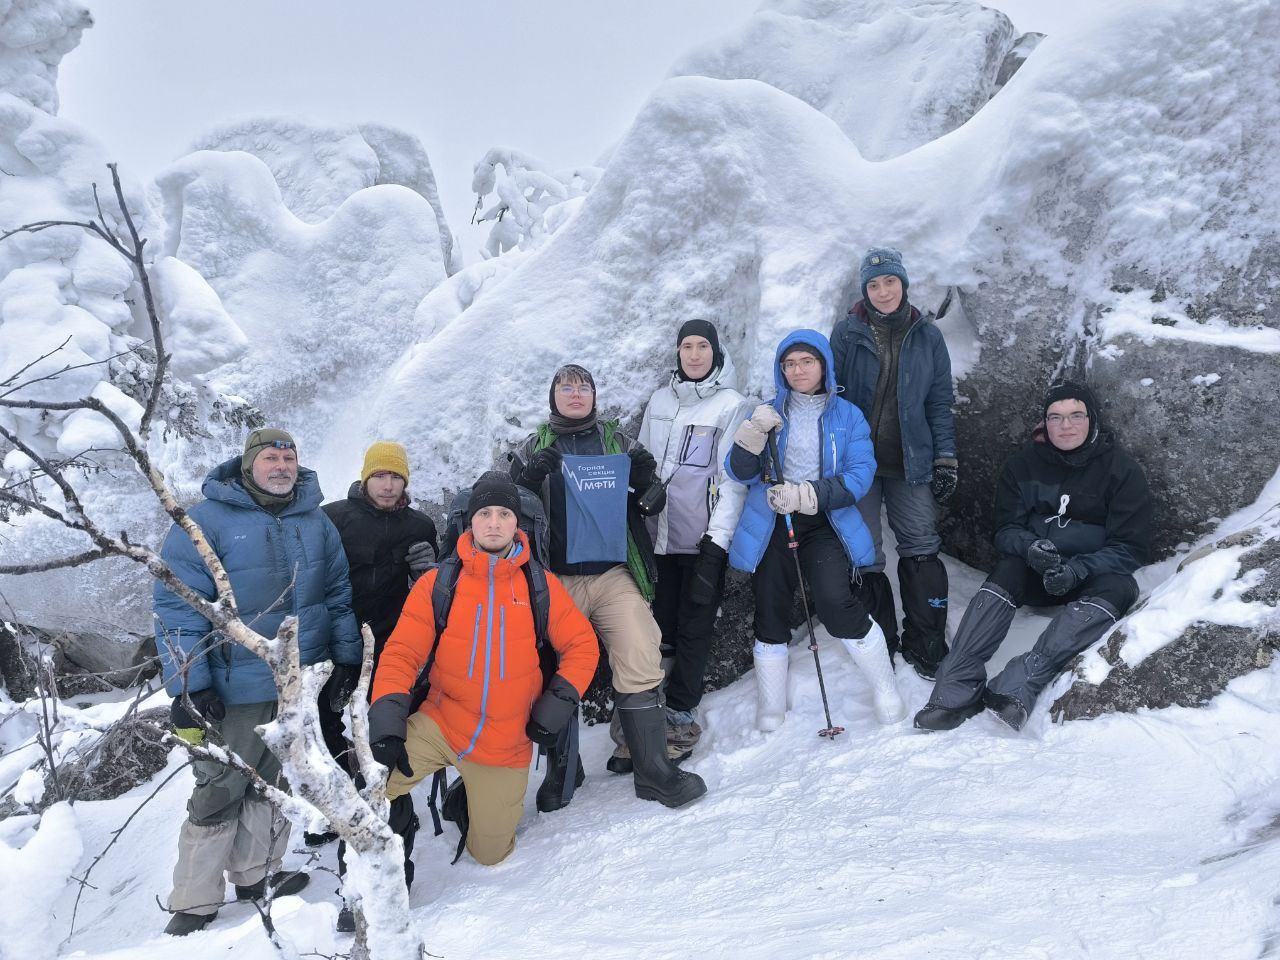
\includegraphics[angle=0, width=0.7\linewidth]{pics/04/perya}
	\caption{Перья. Сразу ясно, откуда такое название}
	\label{fig:perya.jpg}
\end{figure}

\begin{figure}[h!]
	\centering
	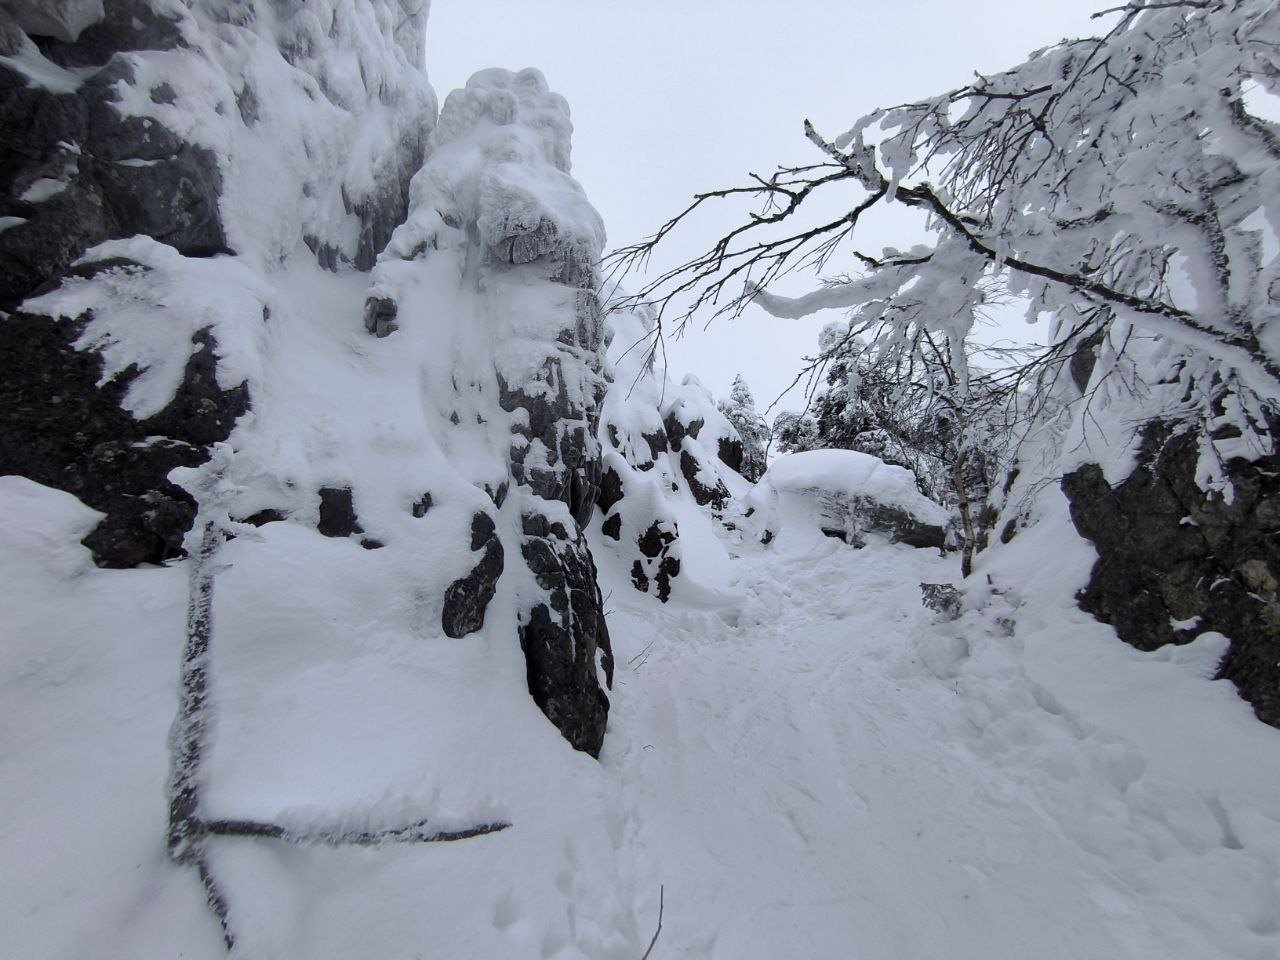
\includegraphics[angle=0, width=0.7\linewidth]{pics/04/near_perya_top}
	\caption{Подступ к вершине. Снова резкая часть подъёма и идти надо осторожно}
	\label{fig:near_perya_top.jpg}
\end{figure}

\begin{figure}[h!]
	\centering
	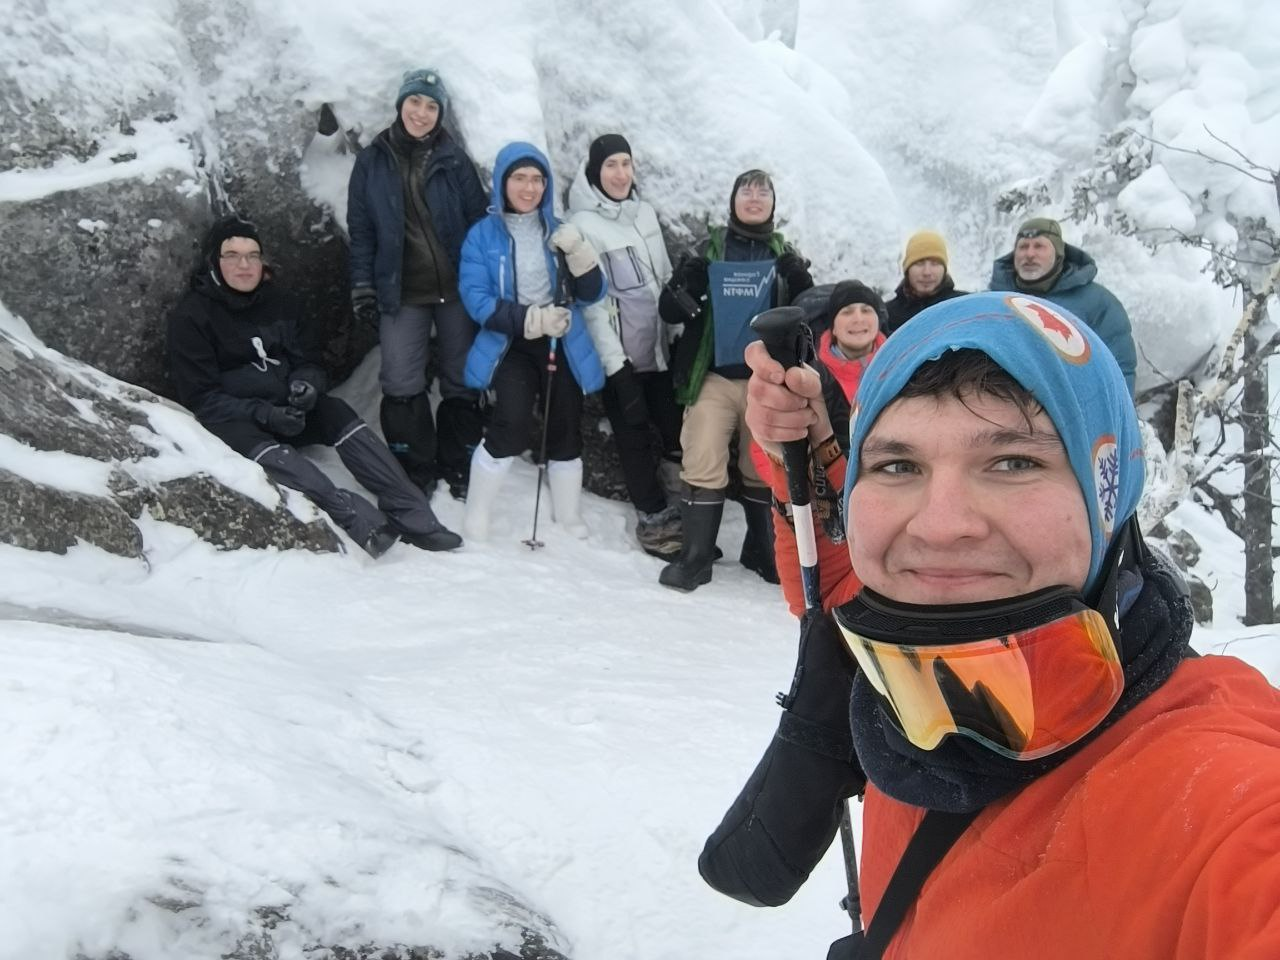
\includegraphics[angle=0, width=0.7\linewidth]{pics/04/perya_top}
	\caption{Добрались! Группа на в. Перья}
	\label{fig:perya_top.jpg}
\end{figure}


По тропе, ведущей вниз, многие туристы спускаются в положении сидя, поэтому идти по ней скользко. В бахилах оказалось удобнее шагать по сугробам (дает достаточно сцепления).

\begin{figure}[h!]
	\centering
	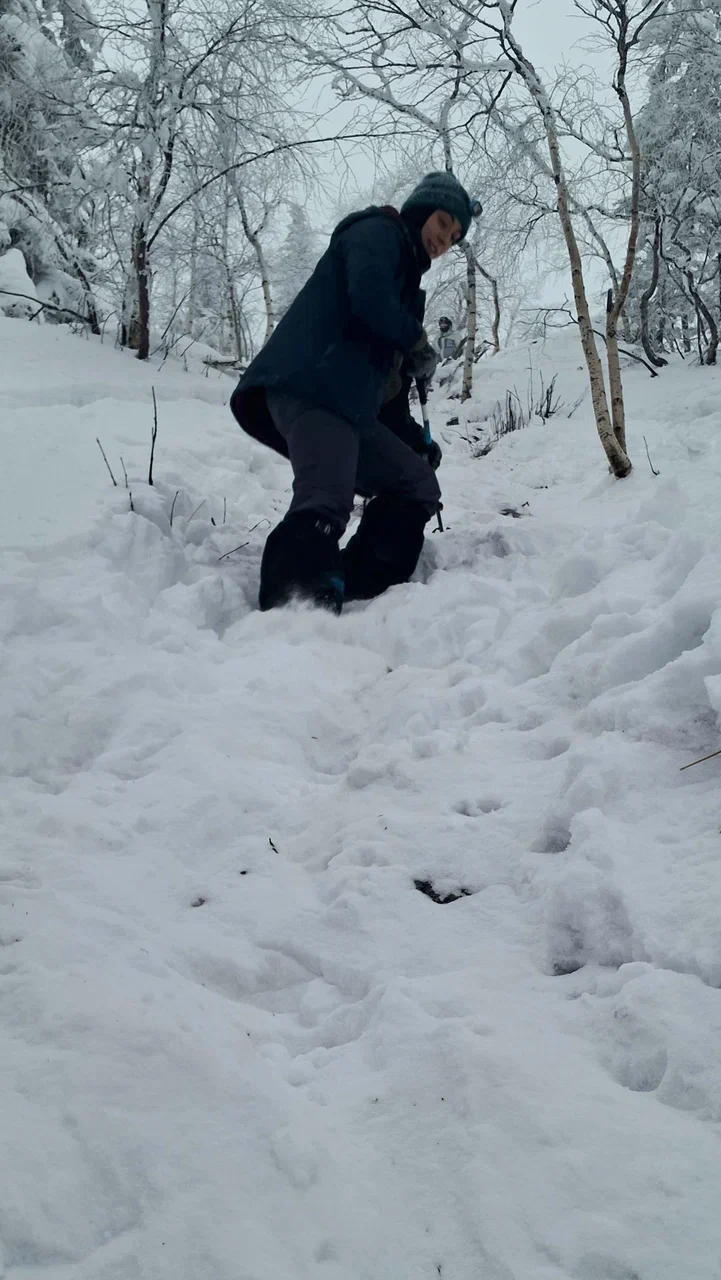
\includegraphics[angle=0, width=0.45\linewidth]{pics/04/down_from_perya}
	\caption{Осторожно спускаемся и почти не падаем}
	\label{fig:down_from_perya.jpg}
\end{figure}

Вернулись к Белому ключу за 50 минут. Здесь есть умывальники, туалет и родник с водой, что приятно. Местная печка, однако, не подходит для готовки еды, поэтому готовили ужин на газу. 

\begin{figure}[h!]
	\centering
	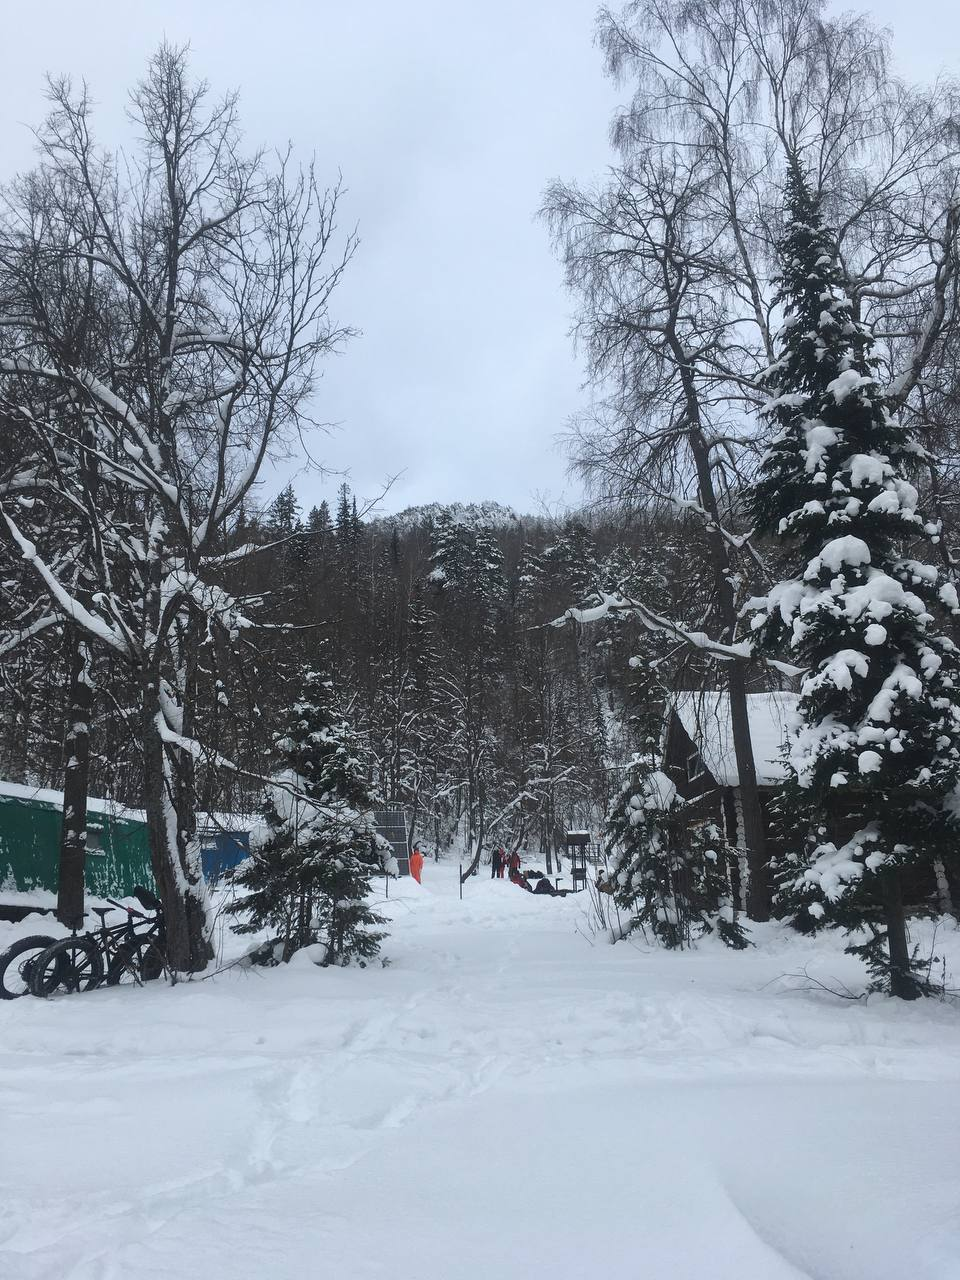
\includegraphics[angle=0, width=0.45\linewidth]{pics/04/Belyi_kliuch}
	\caption{Белый ключ собственной персоной. Милое местечко}
	\label{fig:Belyi_kliuch.jpeg}
\end{figure}

После ужина несколько часов провели в обнимку с лыжами и ремнабором: у 5 участников из 9 камус на носке наглотался снега и отошел, а еще одному пришлось перекручивать плохо затягивающееся крепление на лыже.

Палатка к тому моменту уже давно прогрелась и купленных трёх охапок сухих дров по 300 руб/шт хватило на всю ночь. Печка довольно экономичная, поэтому дежурили раз в 2 часа и на просторных лежанках 

Координаты м.н.: N 55.26398° E 59.77769° 

ЧХВ: 4:50 , ОХВ: 06:23 
\clearpage